\documentclass[11pt, oneside]{article}   	% use "amsart" instead of "article" for AMSLaTeX format
\usepackage{geometry}                		% See geometry.pdf to learn the layout options. There are lots.
\geometry{letterpaper}                   		% ... or a4paper or a5paper or ... 
%\geometry{landscape}                		% Activate for for rotated page geometry
%\usepackage[parfill]{parskip}    		% Activate to begin paragraphs with an empty line rather than an indent
\usepackage{graphicx}				% Use pdf, png, jpg, or eps� with pdflatex; use eps in DVI mode
								% TeX will automatically convert eps --> pdf in pdflatex		
\usepackage{amssymb}
\graphicspath{{/Users/telliott_admin/Dropbox/Tex/png/}}

\title{Difference Quotient}
%\author{The Author}
\date{}							% Activate to display a given date or no date

\begin{document}
\maketitle
%\section{}
%\subsection{}
\large
The basic method for finding the slope of a tangent line to a function $f(x)$ at $x$ is to compute the difference quotient
\[ \frac{f(x+h) - f(x)}{h} \]
for a small change $h$.
\begin{center} 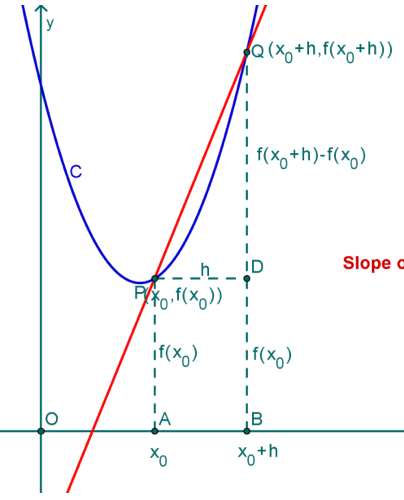
\includegraphics [scale=0.5] {diffQ.png} \end{center}
Here we have some function $f(x)$ in blue, and the first point of interest is $P$, which has its x-coordinate labeled as $x_0$.  The point on the curve at $x=x_0$ is $f(x_0)$, and that is the point plotted as $P$, with coordinates $P=(x_0,f(x_0))$.  Now we move a small distance $h$ away from $x_0$ and compute $f(x_0 + h)$, and call that point $Q$.
 
The slope of the secant line connecting $P$ and $Q$ is $\Delta y / \Delta x$, between the points $(x,f(x))$ and $(x+h, f(x+h))$ on the curve $y=f(x)$.  Since $\Delta x=h$ and  $ \Delta y = f(x + h) - f(x)$, the slope is
\[ \frac{\Delta y}{\Delta x} = \frac{f(x + h) - f(x)}{h} \]

\noindent This is all basic analytical geometry.  Now comes the calculus part.  To find the derivative, which is the slope of the tangent to the curve $f(x)$ \emph{at $x_0$}, we imagine moving the point $Q$ closer and closer to $P$, without every quite getting there, but very, very close.  We compute the limit
\[ \lim_{h \to 0}  \  \frac{f(x+h) - f(x)}{h}  \]
The simplest example is $f(x) = x^2$.  Then we have
\[ slope = \lim_{h \to 0} \frac{f(x+h) - f(x)}{h} \]
\[ \frac{f(x+h) - f(x)}{h} = \frac{x^2 + 2xh + h^2 - x^2}{h} = \frac{2xh + h^2}{h} = 2x + h \]
\[ \lim_{h \to 0}  \  2x + h = 2x  \]
At every point on the curve $y=x^2$, the slope of the tangent line to the curve is $2x$.  We call this process of computing the difference quotient and then taking the limit as $h \to 0$, "taking the derivative."  It produces an expression which is the derivative of y with respect to x, in this case
\[ \frac{dy}{dx} = 2x \]
Another useful shorthand uses the $f$ from $f(x)$, where we adopt the notation that the derivative of $f(x)$ is $f'(x)$.

If we repeat this exercise with a leading constant $a$ (that is, for $f(x) = ax^2$), we find that every term in the numerator of the difference quotient will contain $a$, and so the final result will be $2ax$.  And in general
\[ \frac{d}{dx} af(x) = a \frac{d}{dx} f(x) \]

We would like to find a general expression for $f'(x)$, when $f(x) = x^n$ when $n$ is an integer ($n = 1, 2, 3 \cdots$).  Recall that the Binomial Theorem gives the expansion of $(x + h)^n$.  We only need the first three terms.
\[ (x + h)^n = x^n + nx^{n-1}h + \frac{n(n-1)}{2} \ x^{n-2}h^2 + \cdots  \]
Now we compute the difference quotient and find the limit
\[ \frac{f(x+h) - f(x)}{h} \]
\[ \frac{x^n + nx^{n-1}h + \frac{n(n-1)}{2} \ x^{n-2}h^2 + \cdots - x^n}{h} \]
\[ \frac{nx^{n-1}h + \frac{n(n-1)}{2} \ x^{n-2}h^2 + \cdots} {h} \]
\[ nx^{n-1} + \frac{n(n-1)}{2} \ x^{n-2}h + \cdots  \]
 and find the limit
\[ lim_{h \to 0}  \ nx^{n-1} + \frac{n(n-1)}{2} \ x^{n-2}h = nx^{n-1}  \]
This is called the power rule
\[f(x) = x^n, \ \ \ \ f'(x) = nx^{n-1} \]
and the above is a proof that it is correct for integer $n$.

Another question is:  what to do with a sum or difference of polynomials, such as 
\[ f(x) + g(x) \]
If you write out the difference quotient
\[ \frac{ f(x+h) - f(x) + g(x+h) - g(x)}{h} \]
everything can be exactly as before, just grouping all the terms from $f(x)$ and those from $g(x)$ separately.  To write a rule for these cases
\[  [f(x) + g(x)]' = f'(x) + g'(x)  \]
The derivative of the sum is the sum of the derivatives.

There are two more extensions to make, these are to the negative integers $n=-1,-2, \cdots$, and to fractional (rational) powers $n/m$.  We will do the example of $n=-1$ first.
\[ f(x) = \frac{1}{x} \]
The numerator $f(x+h)-f(x)$ is
\[ \frac{1}{x+h} - \frac{1}{x} =  \frac{x - (x+h)}{x(x+h)} = \frac{-h}{x(x+h)} \]
Multiply by $\frac{1}{h}$ for the actual difference quotient
\[ \frac{-1}{x(x+h)}  \]
and find the limit
\[ \lim_{h \to 0} \ \frac{-1}{x(x+h)}  = -\frac{1}{x^2} \]
So we see that $f(x) = x^{-1}$ follows the power rule $f'(x)=nx^{n-1}$.
 
For a rational power I will start with the square root.  We have 
\[ \frac{d}{dx} \sqrt{x} = \lim_{h \to 0} \frac{\sqrt{x + h} - \sqrt{x}}{h} \]
Clean the numerator up by multiplying by
\[ \frac{\sqrt{x + h} - \sqrt{x}}{h} \ \ \frac{\sqrt{x + h} + \sqrt{x}}{\sqrt{x + h} + \sqrt{x}} = \frac{x + h - x}{h \ (\sqrt{x + h} + \sqrt{x}) } = \frac{1}{\sqrt{x + h} + \sqrt{x} }\]
In the limit, this is just
\[ \frac{1}{2 \sqrt{x}}  \]
This follows the power rule
\[ \frac{d}{dx} \sqrt{x} = \frac{d}{dx} x^{1/2} = \frac{1}{2 \sqrt{x}}  \]
For a general rational power $m/n$ I want to show a trick that is somewhat advanced but especially pretty.  It relies on implicit differentiation.
\[ y = x^{\frac{m}{n}} \] 
\[ y^n = x^m \]
\[ ny^{n-1} y' = mx^{m-1} x' \]
\[ \frac{y'}{x'} = \frac{dy}{dx} = \frac{m}{n} \ \frac{ x^{m-1}}{y^{n-1}} \]
Now 
\[ y^{n-1} = x^{\frac{m}{n}(n-1)} \]
If we write all the powers of x in the numerator we have
\[ x^{m-1 - (n-1)\frac{m}{n}} = x^{m - 1 - m + \frac{m}{n}} = x^{\frac{m}{n} - 1}\]
which gives finally
\[ \frac{dy}{dx} = \frac{m}{n} \  x^{\frac{m}{n} - 1} \]
We've shown that powers of x with rational exponents obey the power rule.  In fact $f(x) = x^\pi$ also obeys the power rule, but we don't need to prove that here.

A second way to do this uses another calculus rule that we haven't covered yet, which is the chain rule, as well as the natural logarithm, which we also haven't covered yet..
\[ x^r = e^{\ln(x^r)} \]
\[ \frac{d}{dx} x^r = \frac{d}{dx} e^{\ln(x^r)} = e^{\ln(x^r)} \ \frac{d}{dx} \ln(x^r)\]
and
\[ \frac{d}{dx} \ln(x^r) = \frac{d}{dx} r \ln(x) \]
we have turned the exponent $r$ into a constant, which we know how to deal with
\[ \frac{d}{dx} r \ln(x) = r \frac{d}{dx} \ln(x) = \frac{r}{x} \]
so we have
\[ \frac{d}{dx} x^r = \frac{d}{dx} e^{\ln(x^r)} = e^{\ln(x^r)} \ \frac{d}{dx} \ln(x^r) = \frac{r}{x} \ e^{\ln(x^r)} = \frac{r}{x} \ x^r = rx^{r-1} \]
which is the power rule for rational exponents, proof 2.

If these last two examples confused you, just take my word for it that the power rule works for \emph{all} $n$.
\end{document}  